%	PACKAGES AND OTHER DOCUMENT CONFIGURATIONS
%----------------------------------------------------------------------------------------

\documentclass[letterpaper]{templatecv} % a4paper for A4
\usepackage{hyperref}
\newcommand\skills{ 
~
	\smartdiagram[bubble diagram]{
        \textbf{Data}\\\textbf{Science},
        \textbf{Algorithms},
        \textbf{Big Data},
        \textbf{Computer}\\\textbf{Vision},
        \textbf{Machine }\\\textbf{Learning},
        \textbf{Statistical}\\\textbf{Analysis},
        \textbf{Artificial}\\\textbf{Intelligence}
    }
}

% Programming skill bars
\programming{
{JAVA / 3},
{C++ / 3},
{C / 3},
{Bash shell scripting/ 3},
{SQL / 3},
{Mathematica / 4},
{LaTeX / 5},
{MATLAB / 5},
{R  / 5},
{Python / 5}%,
}
\languages{{Swedish / 1.5},
{English / 6}%,
}
% Projects text
%\projects{

%}

%----------------------------------------------------------------------------------------
%	 PERSONAL INFORMATION
%----------------------------------------------------------------------------------------

\cvname{\Large{DEVOSMITA CHATTERJEE}\\\small{\textcolor{black}{\bf{Permanent Resident of Sweden}}}} % Your name
%\profilepic{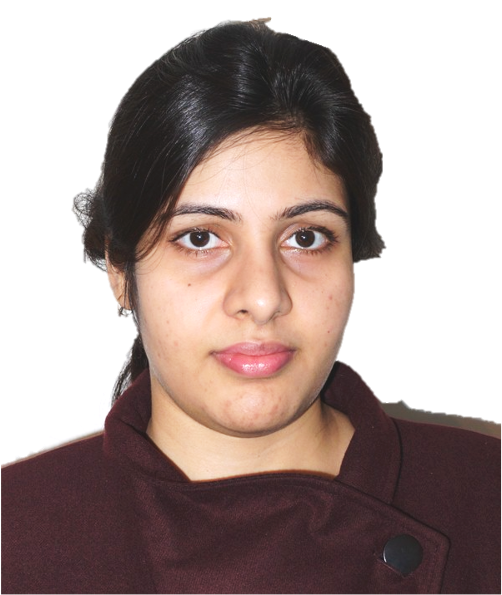
\includegraphics[width=5.2cm, height=5.4cm]{img/Picture 1.png}} % Photo
\cvmap{Wättnegatan 11,   \vskip 5pt 431 39 Mölndal, Sweden}
\cvskype{devosmita.chatterjee}
\cvlinkedin{/in/devosmitachatterjee/}
\cvgithub{devosmitachatterjee2018}
\cvresearchgate{/profile/Devosmita-Chatterjee}
\cvnumberphone{+46 709669519} % Phone number
%\cvsite{} % Personal website
\cvmail{chatterjeedevosmita267
@gmail.com} % Email address

%----------------------------------------------------------------------------------------
\setstretch{1.1}
\begin{document}

\makeprofile % Print the sidebar
\section{Summary}
\begin{itemize}
    \item Engineer with M.Sc in Engineering Mathematics and Computational Science from Chalmers University of Technology, Sweden. Areas of specialization are Statistics, Data Science and Artificial Intelligence.
\item Computational proficiency in Python, Matlab, R, SQL, C and C++.
%\item Native level of English fluency.
%\item Advanced problem solving and troubleshooting ability.
\item Executed projects with Volvo Group and AstraZeneca.
\item Developed an open-source data cleaning standalone application as master thesis project sponsored by Volvo power train department.
\item Extremely sociable personality and great enthusiasm in team building
\end{itemize}
%Aspiring for an ambitious and motivating role in a multicultural work environment. Also striving to be an asset in work team through hard work and perseverance.
 
%----------------------------------------------------------------------------------------
%	 EDUCATION
%----------------------------------------------------------------------------------------

%----------------------------------------------------------------------------------------
%	 EXPERIENCE
%----------------------------------------------------------------------------------------




\section{Projects}
\begin{twenty} 
\twentyitem
    	{Jan 2020 -}
		{Oct 2020}
        {Master Thesis Intern}
        {\href{http://www.volvogroup.com/}{Volvo Group Trucks Technology, Sweden}}
        %{}
        {}
        %{}
        {
Context: Presently, large amount of data generated by organizations drives their business decisions. 
Poor data quality leads to incorrect decisions for the organizations. Data cleaning is a method to solve the data quality issues. But, it is a time consuming task. This demands efficient data cleaning tools for systematically examining data for errors and automatically cleaning them and thus, helps organizations save time and increase their efficiency. \\
Project: The project is about developing a cooperative data cleaning tool. The application can illustrate and address the potential data problems such as inconsistent data, noisy data, outliers, and missing data. It also suggests actions so that users can make informed decisions to clean data effectively.\\
Responsibilities:
\begin{itemize}
\item Coding and developing the open source standalone application ‘DataCleaningTool’.
\item Application design, debugging and deployment.
\item Employ the MissForest imputation method for imputing both missing numerical and categorical values.
\item Create Github repo with proper licensing and a detailed readme file: \\ \href{https://github.com/devosmitachatterjee2018/DataCleaningTool}{https://github.com/devosmitachatterjee2018/DataCleaningTool.}
\item Publish Masters thesis report in Chalmers Open Digital Repository: 
\href{https://odr.chalmers.se/handle/20.500.12380/302324}{https://odr.chalmers.se/handle/20.500.12380/302324.}
\item Work independently.
\end{itemize}

Environment: Windows, Matlab App Designer.    }
      \\
      
      
      \twentyitem
    	{Nov 2019 -}
		{Jan 2020}
		%{}
        {Masters Project Intern}
        {\href{http://www.volvocars.com/}{Volvo Cars, Sweden}}
        {}
        {Context: Ensuring safety of operation is one of biggest challenges for market introduction of autonomous driving vehicles. Autonomous vehicle must manage with any kind of traffic scenario that can possibly occur. Therefore, to verify autonomous driving, the comprehensive set of traffic scenarios needs to be identified. There is need for a mathematical model to determine what should be interpreted as similar scenarios, and what should not be.\\ 
        Project: The project aims to find a model and investigate its capability to identify all possible kinds of complex traffic scenarios around autonomous vehicles.\\
        Responsibilities:
\begin{itemize}
\item Propose a state transition model for describing the traffic scenarios.
\item Describe the surrounding traffic objects in the model by occupation grids. The grids are translated into binary matrices where 1 denotes the
occupation of nearby traffic object. Also attributes such as the vehicle’s speed and angular movement are used.
\end{itemize}}
           \end{twenty}
        \newpage
\makenewprofile
\begin{twenty}
\twentyitem
{}
{}
{}
{}
{}
{
\begin{itemize}
\item Evaluate the model by analysing sequences of states computed from real traffic data provided by Viscando.
\item Use clustering method to distinguish different scenarios represented by the model.
\item Collaborate with two other team members.
\end{itemize} 
Environment: Windows, Python.
   }\\
         \twentyitem
    	{Mar 2019 -}
		{Jun 2019}
		%{}
        {Masters Project Intern}
        {\href{https://www.astrazeneca.com}{AstraZeneca, Sweden}}
        {}
        {Context: For the production of medical tablets, it is important to know how the manufacturing process affects the composition. To do this, one first needs to be able to identify the different components in the tablet based on micro-CT images. %The data for the project has been provided by AstraZeneca. %The tablets are produced with three different methods, namely the direct compression method, the rolling compaction method and the twin-screw granulation method. 
        Image segmentation is used to determine the location and spread of various components in the tablets.\\
        Project: The project is to design a method for distinguishing tablet components in micro-CT images using image segmentation. \\
Responsibilities:
\begin{itemize}
\item Account for image preprocessing, segmentation and analysis.
\item Calculate the share of each component and compare to the theoretical values provided by AstraZeneca.
\item Collaborate with two other team members.
\end{itemize} 
Environment: Windows, Matlab.
   }\\
\twentyitem
   		{Feb 2016 -}
		{Aug 2018}
        {Project Fellow}
        {\href{https://www.iiests.ac.in/}{Indian Institute of Engineering, Science and Technology, India}}
        %{
        {}
        %{
        {Context: Accelerating phase of expansion of the current Universe. \\
        Project: The project is to perform mathematical analysis which leads to the fact that acceleration of the Universe is sustained in the long run. 
        
        Resonsibilities: 
        \begin{itemize}
            \item Study dynamical system of various cosmological models explaining cosmic acceleration.  
            \item Made several successful research collaboration to accomplish project objectives. 
            \item Contribute two high-quality scientific publications.\\ \url{https://doi.org/10.1140/epjp/i2019-12578-1}\\ \url{https://doi.org/10.1007/s12043-018-1544-y}
        \end{itemize}\\
        Environment: Windows, Matlab, Mathematica.

        
   }
     %   }
  %   \\
   %   \twentyitem
   %		{Jul 2015 –}
%	 	{Apr 2017}
 %        {Lecturer}
  %       {\href{https://iem.edu.in/}{Institute of Engineering and Management, India}}
   %      {}
    %     {
     %    {Taught: Mathematics.}}
       \end{twenty}
        
       % \newpage

  %  \\   
  %  \begin{twenty}
    
 %   \\
 %     \twentyitem
 %   		{Jan 2015 –}
% 		{Jun 2015}
%         {Guest Lecturer}
%         {\href{http://www.ecgcollege.org/}{East Calcutta Girls' College, India}}
%         {}
%         {
%         {Taught mathematics in various bachelor degree programs.
%   }
%   }
%   \\
%      \twentyitem
%    		{Nov 2014 –}
% 		{Jun 2015}
%         {Guest Lecturer}
%         {\href{http://www.gurudascollege.edu.in/}{Gurudas College, India}}
%         {}
%         {
%         {Taught mathematics in various bachelor % degree programs.
%   }
%   }


\section{Education}

\begin{twenty} 
	\twentyitem
    	{Sep 2018 -}
        {Aug 2021}
        {M.Sc.}
        {\href{https://www.chalmers.se/en/Pages/default.aspx}{Chalmers University of Technology, Sweden}}
        {\textbf{Engineering Mathematics and Computational Science}}
        {Advanced Differential Calculus [MMA210], Nonlinear Optimization [TMA947], High Performance Computing [TMA881], Scientific Visualization [MVE080], Linear Statistical Models  [MVE190], Statistical Inference [MVE155], %Algorithms [TIN093](in progress), 
        Experimental Design and Sampling [TMS032], Financial Time Series [TMS088], 
        Spatial Statistics and Image Analysis [TMS016], %Statistical Learning for Big Data [MVE440] (in progress), 
        Artificial Neural Networks [FFR135], %Stochastic Optimization Algorithms [FFR105] (in progress),
        Computer Vision [EEN020], Project Course in Mathematical and Statistical Modelling [MVE385], Master's Thesis in Mathematics [MVEX03]}\\
	\twentyitem
    	{Sep 2012 -}
		{Nov 2014}
        {M.Sc.}
        {\href{https://www.caluniv.ac.in/}{Calcutta University, India}}
        {\textbf{Applied Mathematics}}
        {%Abstract Algebra, Classical Algebra, Linear Algebra, Linear Optimization, Ordinary and Partial Differential Equations, Dynamical Systems, Mechanics, Numerical Analysis
        }\\
        \twentyitem
    	{Jul 2009-}
		{Jul 2012}
        {B.Sc.}
         {\href{https://www.sxccal.edu/}{St. Xavier's College, India}}
 {\textbf{Mathematics}}
        {%Algebra, Probability and Statistics, Computer Programming
        }

\end{twenty}

\end{document} 
